\documentclass[a4paper]{article}

\usepackage[english]{babel}
\usepackage[utf8]{inputenc}
\usepackage{float}
\usepackage{amsmath}
\usepackage{graphicx}
\usepackage{subfigure}
\usepackage[colorinlistoftodos]{todonotes}

\title{\bfseries{COMP90016 -- Assignment 1 }}
\author{Haonan Li}

\date{\today}

\begin{document}
\maketitle

\section{Introduction}
\label{sec:introduction}

This assignment consists of three tasks. 

For the first task, we first build a k-mer index for a reference file, then aligned all reads from a FASTQ reads file using the index.

The second task is to investigate the runtime of the aligner build in task 1. In this task, we compare the speed of the new aligner with the naive aligner proposed in group assignment. In addition, we also evaluate the realation between size of k-mer and the alignment speed.

For the last task, we extend our algorithm to further investigate mismatches to the reference.

\section{Results \& Discussion}
\label{sec:experiment}
\subsection{Task 2}

\begin{table}[H]
	\centering
	\begin{tabular}{c|c|c|c|c|c|c|c}
		\hline
		k & 0 & 4 & 8 & 13 & 16 & 32 & 50 \\
		\hline
		ref1 & 24.43 & 18.98 & 1.76 & 1.48 & 1.40 & 1.04 & 0.51 \\
		\hline
		ref2 & 50.87 & 35.34 & 1.83 & 1.49 & 1.49 & 1.14 & 0.66 \\
		\hline
		ref3 & 80.54 & 52.65 & 1.91 & 1.56 & 1.47 & 1.22 & 0.78\\
		\hline
	\end{tabular}
	\caption{\label{tab:1}Time consuming for k-mer indexed alignment. (k=0, refers to  the naive aligner.)}
\end{table}

\begin{figure}[!htb]
	\centering
	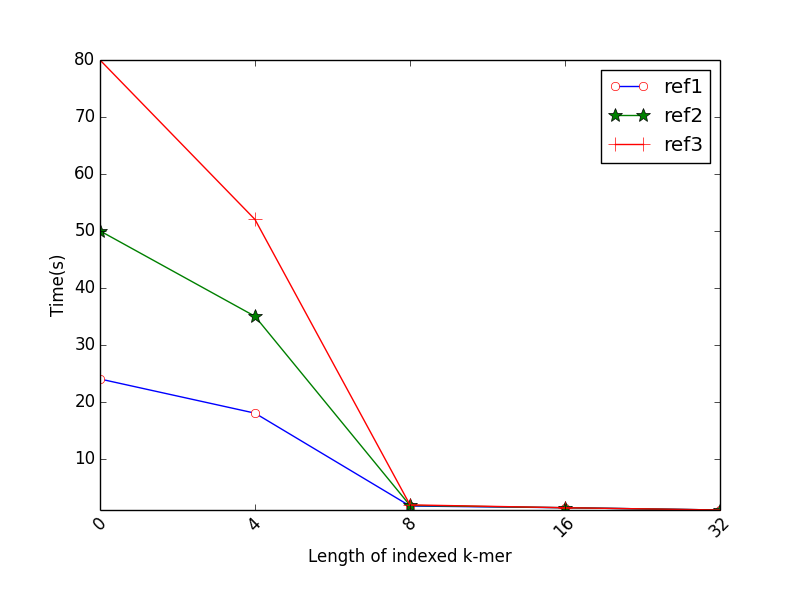
\includegraphics[width=0.5\textwidth]{align_time.png}
	\caption{\label{fig:1}Time consuming for k-mer indexed alignment. (k=0, refers to  the naive aligner.}
\end{figure}

Table \ref{tab:1} and Figure \ref{fig:1} show the time comsuming for k-mer aligner work on the given datasets. K=0 refers to the naive aligner proposed in group assignment. From these results, we find that new aligner is much more effcient than the naive alignments. As the increase of k, the speed of alignment increase. For a samll k ($k<6$), the change is obvious. But if k is large ($k>8$), the accelerate become less obviously.

The result is not surprised. Because the  complexity of naive Hamming distance aligner is O(ngl), where n is the number of reads, g the length of the genome, and l the length of the reads. But for indexed aligner, the complexity is O(nlp), where p is the average number indexes for each k-mer, it is depend on the length of k and ref. Because the number of different k-mer for a vertain k is $2^k$. If the k is large, the complexity of k-mer indexed aligner could be O(nl).

\subsection{Task 3}

FIgure \ref{a}  shows the distribution of base quality scores of all the reads for each position, and Figure \ref{b} the distributions of quality scores of all mismatches for alignment to the given reference ref1.fa  (also by position). 

Compare these two images, we find that the range of each position's quality score of two piecture is almost the same, whis indicates even a position have a high average quality score or most quality scores of this position is high, mismatch also happened. We also find that the upper quartile are almost the same in these two pictures for the same position. However, the lower quartile and median show some different. For all positions, the lower quatile of mismatched picture always less than the statistics for all reads. This is due to more low quality scores appear in the mismatched set.  
Besides, as the position vary form 1 to 100, the average quality score become lower and lower, mismatches increase. This was reflected by the median lines, they overlap the bottom of the picture for most positions near to 100.

\begin{figure}[!htb]
	
	\centering
	\subfigure[All the reads for each position]{
		\label{a} 
		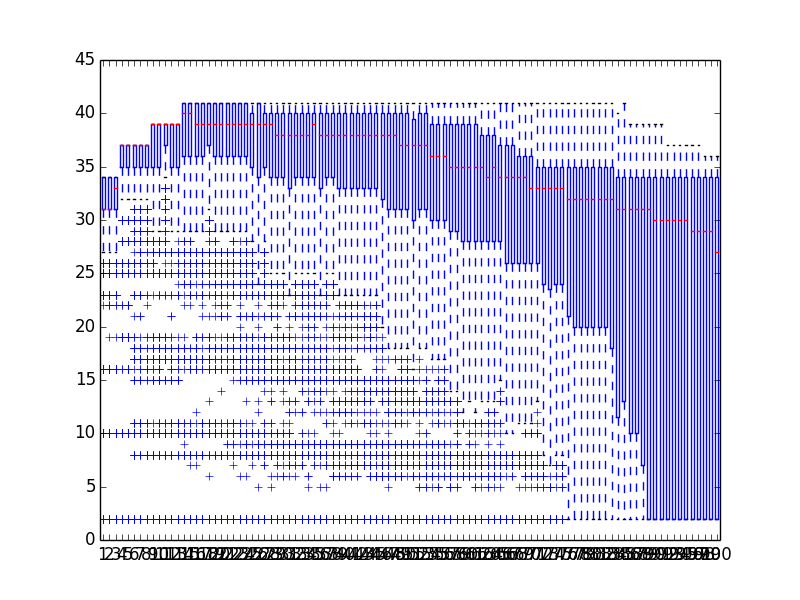
\includegraphics[width=0.4\textwidth]{base_qs.png}}
	\hspace{0.5in}
	\subfigure[All mismatches]{
		\label{b} 
		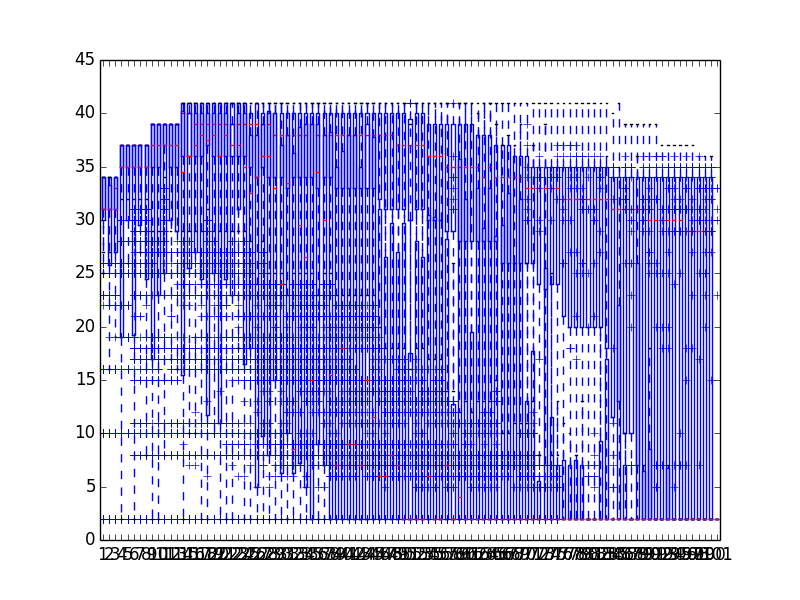
\includegraphics[width=0.4\textwidth]{mis_qs.png}}
	\caption{Distribution of base quality scores.}
	\label{fig:2} 

\end{figure}
 


%\begin{thebibliography}{9}
%\end{thebibliography}
\end{document}